\documentclass{article}
\usepackage[utf8]{inputenc}
\usepackage[spanish]{babel}
\usepackage{amsmath}
\usepackage{amssymb}
\usepackage{amsfonts}
\usepackage{hyperref}
\usepackage{textcomp}
\usepackage{graphicx}
\usepackage{pgfplots}
\usepackage{geometry}
\usepackage{booktabs}
\hypersetup{
    colorlinks=true,
    linkcolor=black,
    citecolor=green,
    filecolor=magenta,      
    urlcolor=cyan,
}
\geometry{
  top=3cm,
  bottom=3cm,
  left=3cm,
  right=3cm
}

\title{Estadística 1}
\author{Jorge Miguel Alvarado Reyes}
\date{16 Agosto 2023}

\setlength{\parindent}{0pt}
\begin{document}

\begin{titlepage}
    \begin{center}
        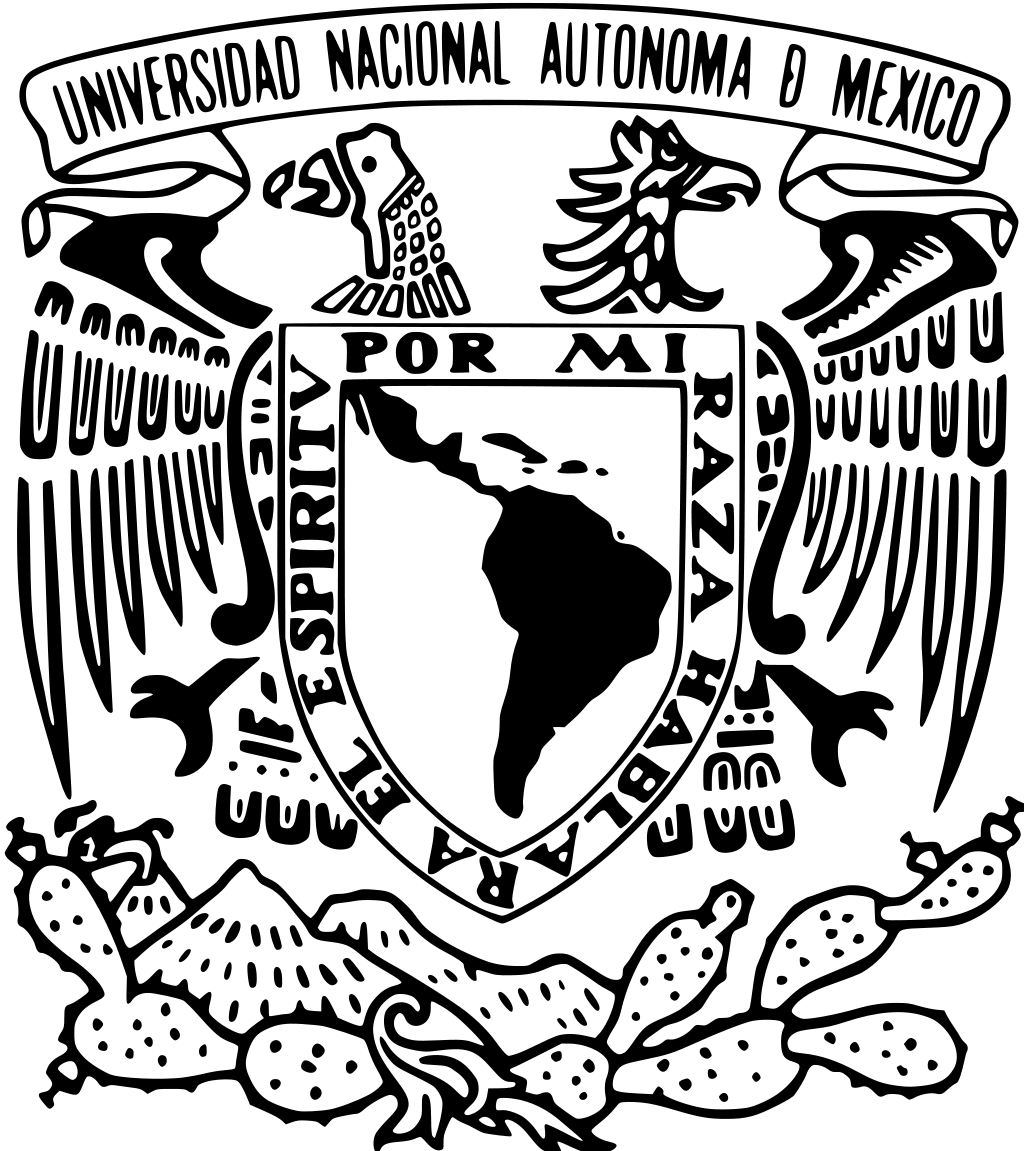
\includegraphics[width=0.2\textwidth]{../../unam.png}
        \vspace*{.5cm}

        \LARGE
        \textbf{Universidad Nacional Autónoma de México}

        \vspace{0.5cm}
        \LARGE
        Facultad de Estudios Superiores Acatlán

        \vspace{2cm}

        \textbf{Estadística 2} \\
        Tarea unidad 1

        \vfill

        \vspace{1cm}

        \textbf{\large Autor:} \\
        Jorge Miguel Alvarado Reyes \\
        \vspace{.5cm}
        \normalsize \today

    \end{center}
\end{titlepage}
\newpage

\tableofcontents

\newpage

\section{Problema 1}
\section{Problema 2}
\section{Problema 3}
\section{Problema 4}
Dos métodos para controlar el tránsito, A y B, se usaron en cada una de n = 12 cruceros durante una semana y los números de accidentes que ocurrieron durante ese tiempo se registraron. El orden de uso (cuál se emplearía para la primera semana) se seleccionó de una manera aleatoria. Se desea saber si los datos dan suficiente evidencia para indicar una diferencia en las distribuciones de porcentajes de accidentes para los métodos A y B de control de tránsito.

\begin{center}
    \begin{tabular}{c c c |c c c}
        Crucero & A & B & Crucero & A & B \\
        \hline
        1       & 5 & 4 & 7       & 2 & 3 \\
        2       & 6 & 4 & 8       & 4 & 1 \\
        3       & 8 & 9 & 9       & 7 & 9 \\
        4       & 3 & 2 & 10      & 5 & 2 \\
        5       & 6 & 3 & 11      & 6 & 5 \\
        6       & 1 & 0 & 12      & 1 & 1 \\
    \end{tabular}
\end{center}

\subsection*{Solución}
Dado que tenemos datos en pares y lo que buscamos demostar es si la distribucion de los datos diferen podemos utilizar una prueba Wilcoxon

\begin{center}
    \begin{tabular}{c c c c c}
        Linea A & Linea B & $| A - B|$ & Rango & R con signo \\
        \hline
        5       & 4       & $|-1|$     & 4     & -4          \\
        6       & 4       & $|2|$      & 8     & 8           \\
        8       & 9       & $|-1|$     & 4     & -4          \\
        3       & 2       & $|-1|$     & 4     & -4          \\
        6       & 3       & $|-3|$     & 8     & -8          \\
        1       & 0       & $|1|$      & 4     & 4           \\
        2       & 3       & $|-1|$     & 4     & -4          \\
        4       & 1       & $|-3|$     & 11    & -11         \\
        7       & 9       & $|-2|$     & 8     & -8          \\
        5       & 2       & $|-3|$     & 11    & -11         \\
        6       & 5       & $|-2|$     & 8     & -8          \\
        1       & 1       & $|0|$      & 1     & 1           \\
    \end{tabular}
\end{center}

\[T_{+} = 8+4+1 = 13\]
\[T_{-} = 4+8+11 = 23\]
\[T = min(T_{+}, T_{-}) = 13\]

\[
    E(T) = \frac{n(n + 1)}{4} = \frac{12(12 + 1)}{4} = 39
\]
\[
    Var(T) = \frac{n(n + 1)(2n + 1)}{24} = \frac{12(12 + 1)(2(12) + 1)}{24} =162.5
\]
\[
    z = \frac{T - E(T)}{\sqrt{Var(T)}} = \frac{13 - 39}{\sqrt{162.5}} = -2.0396
\]

Tomando $\alpha = 0.05$

\[q_z(1 - \frac{\alpha}{2}) = 1.96\]

Se rechaza $H_0$ si

\[|z| > q_z()\]

\[2.0396 > 1.96\]

Por lo tanto las funciones de densidad son diferentes

\begin{center}
    \begin{tabular}{c c c c c}
        Linea A & Linea B & $| A - B|$ & Rango & R con signo \\
        \hline
        5       & 4       & $|1|$      & 3.5   & 3.5         \\
        6       & 4       & $|2|$      & 7.5   & 7.5         \\
        8       & 9       & $|-1|$     & 3.5   & - 3.5       \\
        3       & 2       & $|1|$      & 3.5   & 3.5         \\
        6       & 3       & $|3|$      & 10    & 10          \\
        1       & 0       & $|1|$      & 3.5   & 3.5         \\
        2       & 3       & $|-1|$     & 3.5   & -3.5        \\
        4       & 1       & $|3|$      & 10    & 10          \\
        7       & 9       & $|-2|$     & 7.5   & -7.5        \\
        5       & 2       & $|3|$      & 10    & 10          \\
        6       & 5       & $|1|$      & 3.5   & 3.5         \\
        1       & 1       & $|0|$      &       &             \\
    \end{tabular}
\end{center}

\[T_{+} = 3.5+7.5+3.5+10+3.5+10+10+3.5 = 13\]
\[T_{-} = 3.5+3.5+7.5 = 14.5\]
\[T = min(T_{+}, T_{-}) = 14.5\]

\[
    E(T) = \frac{n(n + 1)}{4} = \frac{11(11 + 1)}{4} = 33
\]
\[
    Var(T) = \frac{n(n + 1)(2n + 1)}{24} = \frac{11(11 + 1)(2(11) + 1)}{24} =126.5
\]
\[
    z = \frac{T - E(T)}{\sqrt{Var(T)}} = \frac{14.5 - 33}{\sqrt{126.5}} = -1.64485
\]

Tomando $\alpha = 0.05$

\[q_z(1 - \frac{\alpha}{2}) = 1.96\]

Se rechaza $H_0$ si

\[|z| > q_z()\]

\[1.64485 > 1.96\]

Por lo anto las dstribuciones son iguales

\section{Problema 5}
Los resultados de un experimento para investigar el reconocimiento de productos, durante tres campañas publicitarias, se muestran en la siguiente tabla. Las respuestas fueron el porcentaje de 400 adultos que estaban familiarizados con el producto recién anunciado. La gráfica de probabilidad normal indicó que los datos no eran aproximadamente normales y debía usarse otro método de análisis. ¿Hay una diferencia significativa entre las tres distribuciones poblacionales de donde vinieron estas muestras?


\begin{center}
    \begin{tabular}{c |c |c}
        \multicolumn{3}{c}{Campaña} \\
        \hline
        1   & 2   & 3               \\
        .33 & .28 & .21             \\
        .29 & .41 & .30             \\
        .21 & .34 & .26             \\
        .32 & .39 & .33             \\
        .25 & .27 & .31             \\
    \end{tabular}
\end{center}


\section{Problema 6}
\section{Problema 7}
\section{Problema 8}
\section{Problema 9}
\section{Problema 10}
\end{document}
